\section{Validity of Augmented Data}

In the process of assessing the augmented data obtained from frequency sequences, it was imperative to ensure the integrity and reliability of the generated data. Several validation steps were conducted to verify the fidelity and accuracy of the augmented dataset.\\

\noindent Initially, the integrity of the augmented data was confirmed by comparing the original dataset with the manipulated dataset. This involved a series of normalization procedures applied to the sequences. Notably, the normalization involved raising the values to the power of 5 and scaling the data with respect to the absolute maximum value in the sequence. Subsequently, a comparative analysis was executed between the original and normalized datasets to ensure consistency and validity.\\

\noindent Moreover, the symmetry of the augmented data was evaluated by determining the barycenter of the normalized sequences. This process involved identifying the index representing the median value within the sequence. Additionally, to confirm symmetry, the dataset was divided into two halves, and their correspondence was examined to check if the sequence was symmetrical with respect to its barycenter.
The assessment of the symmetry involved summing the absolute values of the first and second halves of the dataset. Comparing these sums was crucial in confirming the symmetry of the sequence. The comparison provided valuable insights into the symmetrical properties of the augmented data, which further reinforced its validity and reliability.\\

\vspace*{0.4cm}
\noindent Here is the graphical representation of the normalization for the ax axis of one recording :
\vspace*{0.3cm}

\begin{figure}[H]
    \begin{adjustbox}{minipage=0.4\textwidth}
    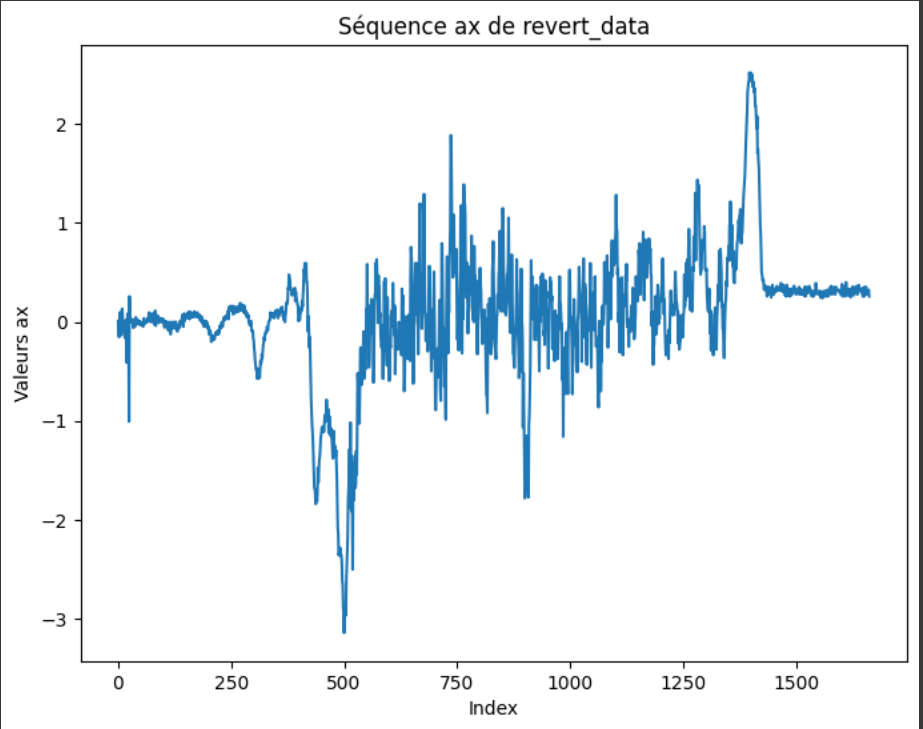
\includegraphics[scale=0.6]{img/reversed_data_ax.png}
    \caption{Initial reversed sequence of ax revert\_data}
    \label{reversed_data_ax}
    \end{adjustbox}
    \hspace*{0.1\textwidth}
    \begin{adjustbox}{minipage=0.4\textwidth}
    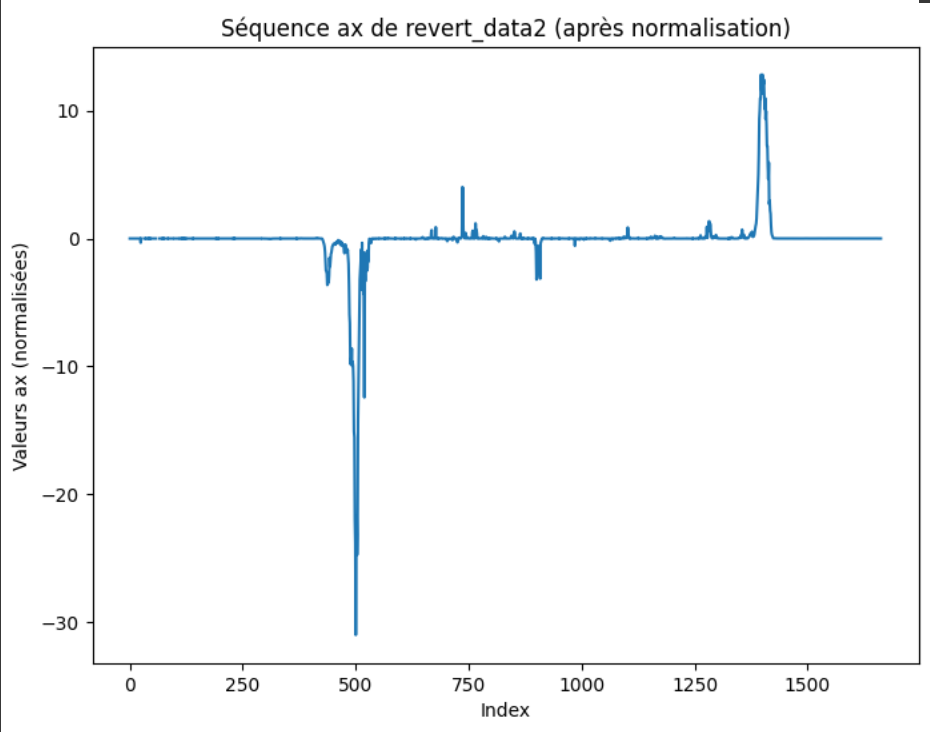
\includegraphics[scale=0.6]{img/reversed_data_ax_norm.png}
    \caption{Normalized reversed sequence of ax revert\_data}
  \label{reversed_data_ax_norm}
    \end{adjustbox}
\end{figure}

\noindent The verification process conducted on the augmented frequency sequences indicated that the generated data preserves essential characteristics of the original dataset. This procedure significantly enhances the confidence in the augmented data's applicability and utility for subsequent analyses and machine learning applications.\\